% ex: ts=2 sw=2 sts=2 et filetype=tex
% SPDX-License-Identifier: CC-BY-SA-4.0
\begin{frame}
    \frametitle{Contenido}
    \tableofcontents
\end{frame}

\section{Python}

\begin{frame}[c]{¿Qué es Python?}
    \begin{columns}
        \column{0.5\textwidth}
        Python es un lenguaje de programación interpretado cuya filosofía hace
        hincapié en la legibilidad de su código. Se trata de un lenguaje de
        programación multiparadigma, ya que soporta parcialmente la orientación
        a objetos, programación imperativa y, en menor medida, programación
        funcional. Es un lenguaje interpretado, dinámico y multiplataforma. 
        \column{0.5\textwidth}
        \begin{center}
            
\includegraphics[scale=0.2]{python-logo.png}
        \end{center}
    \end{columns}
\end{frame}

\begin{frame}[c]{Historia}
  \begin{columns}
    \column{0.7\textwidth}
    \begin{itemize}
      \item Creado por Guido Van Rossum
      \item Holanda finales de la decade de los 80's
      \item Sintaxis simple, práctica e intuitiva
      \item De proposito general: NASA, motor de busqueda de Google, Bolsa de
        Valores de Nueva York
      \item Interpretado
      \item Multiparadigma
      \item Tipado dinámico
      \item Python 2.X ya esta descontinuado, solo hay que usar el 3.X
    \end{itemize}
    \column{0.3\textwidth}
        \begin{center}
            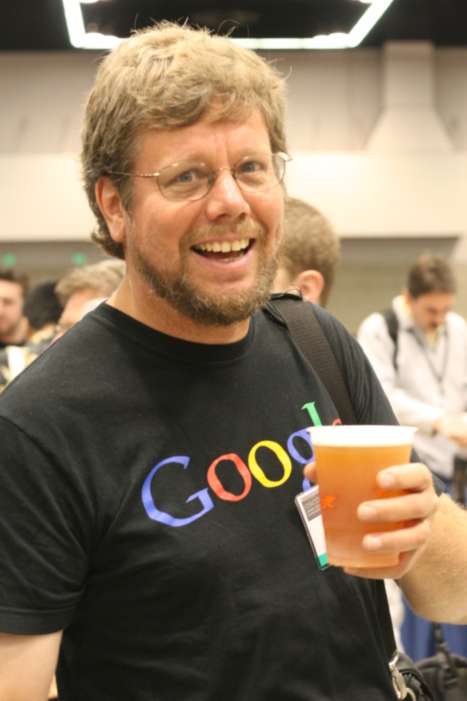
\includegraphics[scale=0.05]{Guido_van_Rossum_OSCON_2006.jpg}
        \end{center}
  \end{columns}
\end{frame}

\begin{frame}[c]{Reglas de codificación}
  \begin{itemize}
    \item Los comentario de una línea inician con "\#"
    \item Los comentarios de varias líneas inician con """ y terminan con """
    \item La sangria cuenta
    \item No poner signos de putuación al final de la instrucción
    \item Es sensible a mayúsculas
    \item Errores de programación:
          \begin{itemize}
            \item Sintaxis
            \item Ejecución
            \item Lógicos
          \end{itemize}
  \end{itemize}
\end{frame}

\begin{frame}[c]{Ejecución de programas}
  \begin{itemize}
    \item El código generado en Lenguaje Python se almacena en un archivo con
      extensión .py
  \end{itemize}
\end{frame}

\section{Pycharm}

\begin{frame}[c]{¿Qué es Pycharm?}
    \begin{columns}
        \column{0.5\textwidth}
        PyCharm es un entorno de desarrollo integrado (IDE) utilizado en
        programación de computadoras, específicamente para el lenguaje Python.
        Está desarrollado por la empresa checa JetBrains (antes conocida como
        IntelliJ).
        \column{0.5\textwidth}
        \begin{center}
            
\includegraphics[scale=0.1]{pycharm-logo.png}
        \end{center}
    \end{columns}
\end{frame}

\begin{frame}[c]{Pantalla de inicio}
    \begin{center}
        Pantalla de inicio
    \end{center}
\end{frame}
